\section{Tutorial}\label{sec:tutorial}
\subsection{Before the simulation: what to do}\label{subsec:before}
Let us see in practice what we have previously learnt in a simple tutorial:
first of all, we need the whole program, available at \url{https://github.com/BFSteam/memory.}\\
Once downloaded it is convenient to put \texttt{path\_to/memory/src} inside
\texttt{path\_to\_SLAPP3/project.txt} as described in \textit{SLAPP\_Reference\_Handbook.pdf pag20}.
Inside SLAPP3 we can run the program \texttt{runShell.py} from terminal
or from jupyter notebook using \texttt{iRunShell.ipynb}.
The program asks which project we want to run: if we set up the path correctly
we can confirm \textit{memory} path and project.
Afterwards we have to set all the necessary input variables to start
the simulation:
\begin{itemize}
\item[\texttt{Random number seed:}] insert the seed to make the simulation reproducible.
\item[\texttt{Number of sources:}]insert the number of sources inside the network.
\item[\texttt{Number of users:}]insert the number of users inside the network.
\item[\texttt{Average degree for users:}]insert the value of the average degree for users only.
\item[\texttt{Number of cycles:}]insert the maximum number time can reach.
\end{itemize}

In order to simplify our first approach, default values are provided:
answering enter at each line will make the program run, and that's it!\\

\subsection{During the simulation: where to put the accent}\label{subsec:during}
Simulation is running and our network is evolving. A window will appear
with the drawing network\footnote{Graphs drawn using
  \href{https://networkx.github.io/}{networkx} and
  \href{https://matplotlib.org/}{matplotlib}}
and flowing time is displayed in terminal. \\
Nodes of the network are painted with different colors: if they don't
spread, gray for inactive state and blue for active one; if they spread can be orange, pink or cyan depending on the spreaded news.
In detail, every source initially generates a single news, tracked by its color. The source's size are bigger than users and labeled with 0,1 and 2; numbering goes on with users.\\
We show network dynamic in the pictures below:
\begin{figure}[!h]
  \centering
  \begin{subfigure}[t]{.45\textwidth}
    \centering
    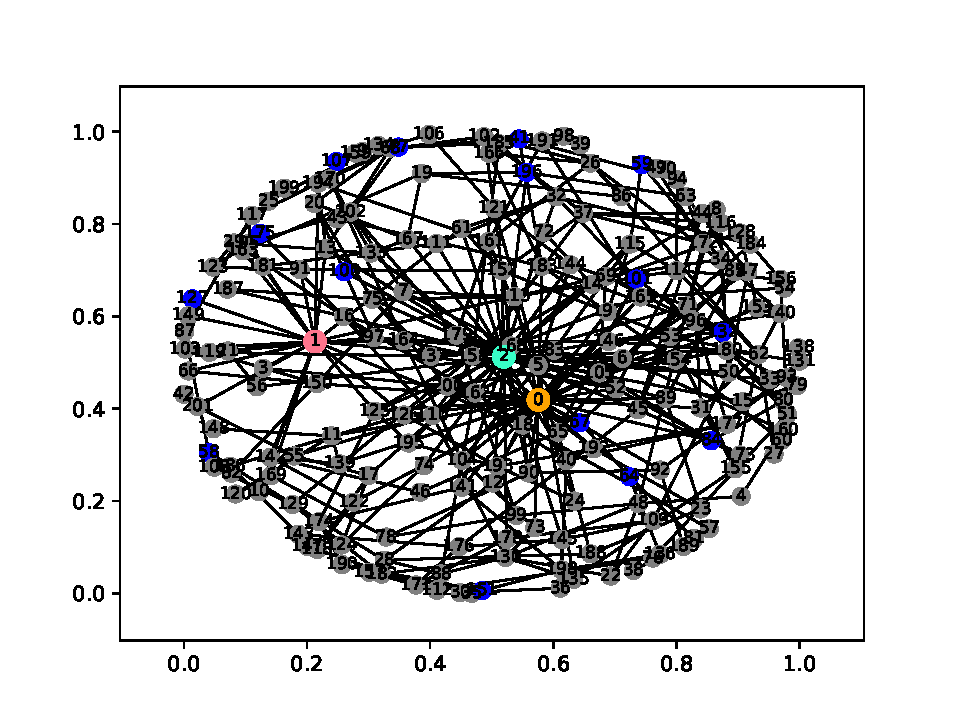
\includegraphics[trim={1cm .5cm 1cm 1cm}, clip, width=\linewidth]{img/pdf/plot-0001.pdf} 
    \caption{1 cycle}
    \label{fig:1}
  \end{subfigure}
  \begin{subfigure}[t]{.45\textwidth}
    \centering
    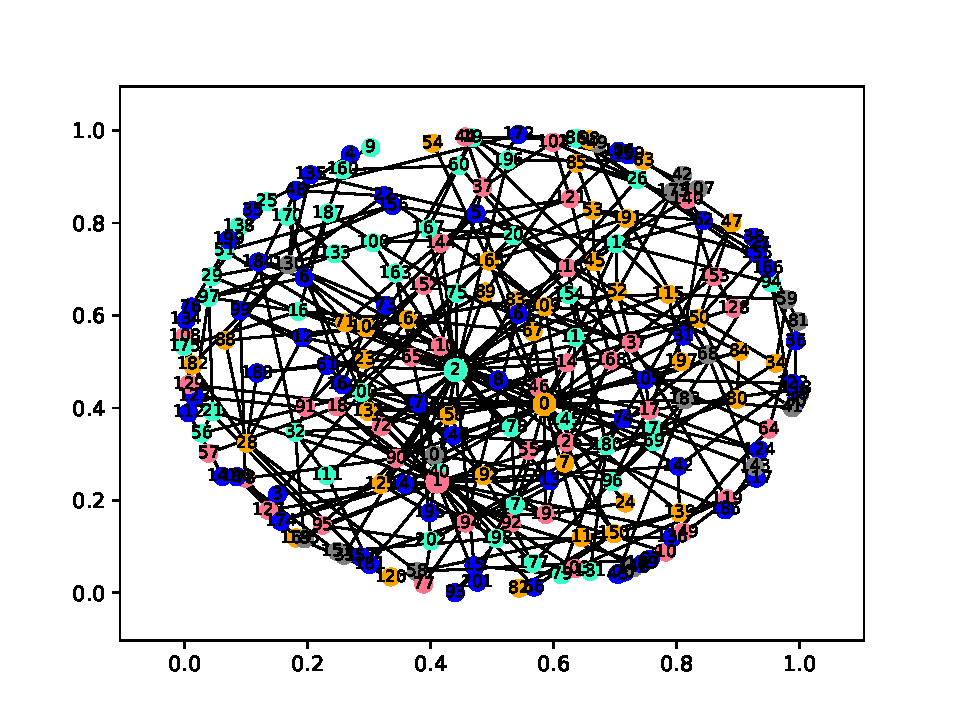
\includegraphics[trim={1cm .5cm 1cm 1cm}, clip, width=\linewidth]{img/pdf/plot-0005.pdf} 
    \caption{5 cycles}
    \label{fig:5}
  \end{subfigure}

  \vspace{0cm}

  \begin{subfigure}[t]{.45\textwidth}
    \centering
    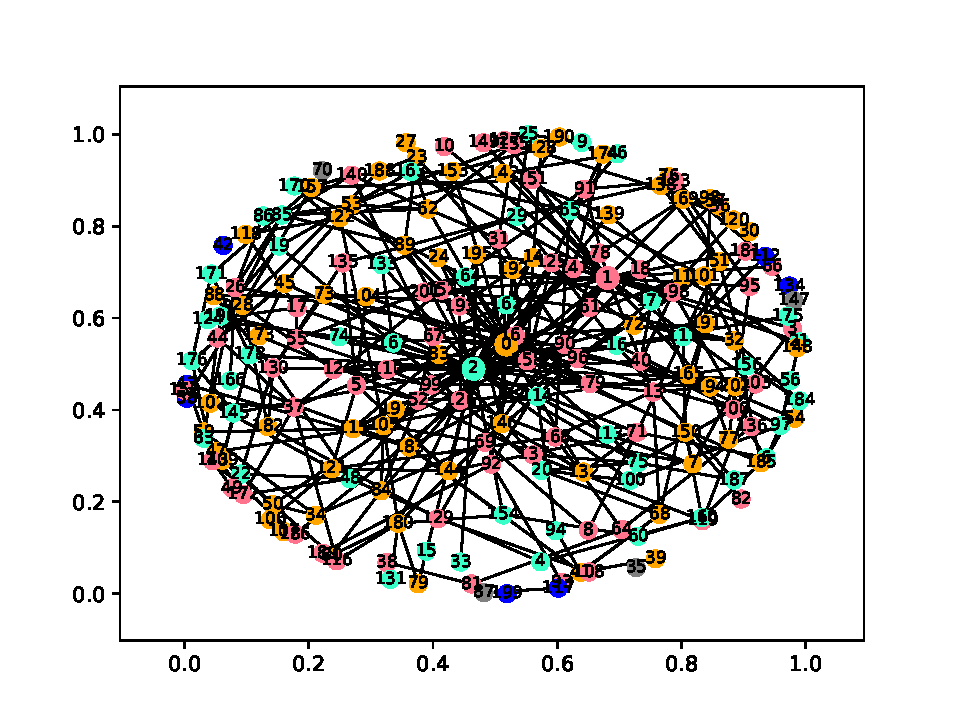
\includegraphics[trim={1cm .5cm 1cm 1cm}, clip, width=\linewidth]{img/pdf/plot-0010.pdf} 
    \caption{10 cycles}
    \label{fig:10}
  \end{subfigure}
  \begin{subfigure}[t]{.45\textwidth}
    \centering
    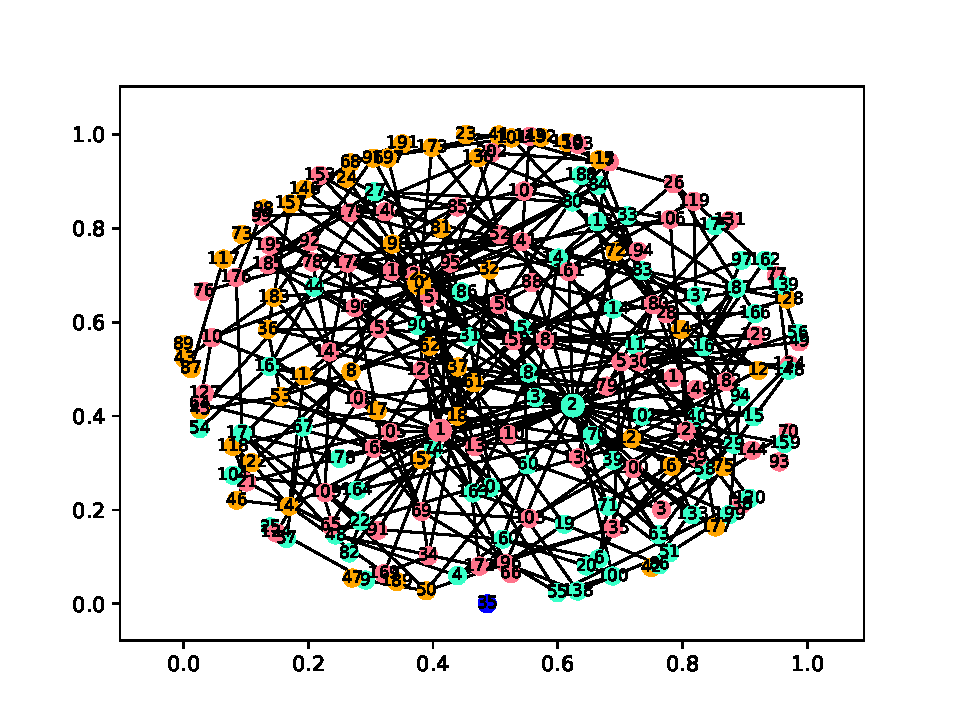
\includegraphics[trim={1cm .5cm 1cm 1cm}, clip, width=\linewidth]{img/pdf/plot-0050.pdf} 
    \caption{50 cycles}
    \label{fig:50}
  \end{subfigure}
 
  \caption{Plot at different initial time steps for a simulation with 3 sources, 200 users, initial average degree of users 3 and 500 time steps. Random seed initialized to 17.}
\end{figure}

\begin{figure}
  \centering
  \begin{subfigure}[t]{.45\textwidth}
    \centering
    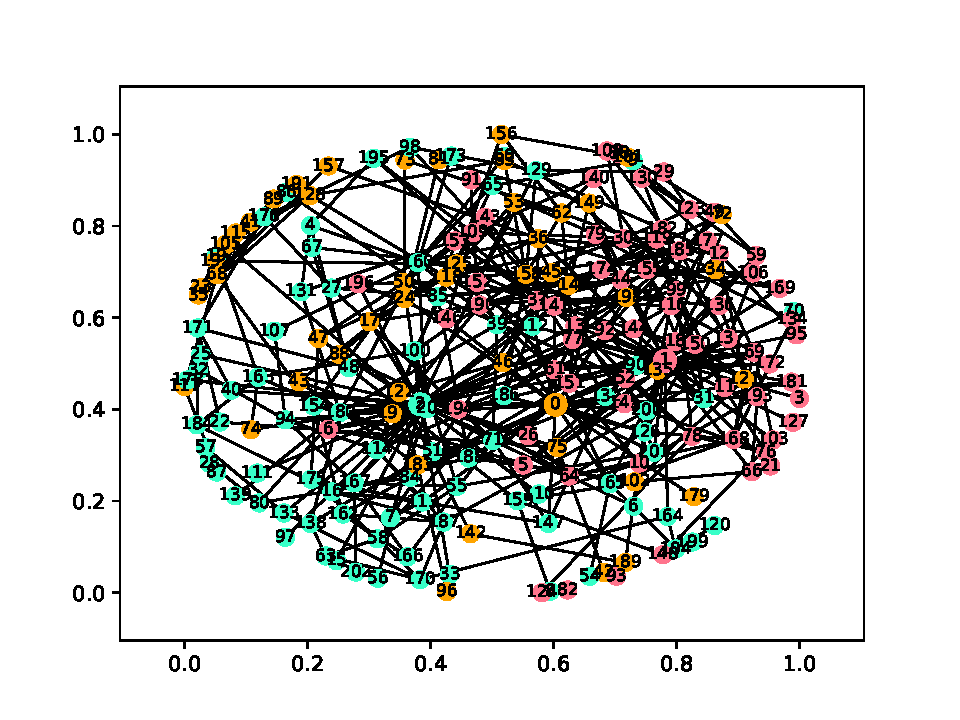
\includegraphics[trim={1cm .5cm 1cm 1cm}, clip, width=\linewidth]{img/pdf/plot-0100.pdf} 
    \caption{100 cycles}
    \label{fig:100}
  \end{subfigure}
  \begin{subfigure}[t]{.45\textwidth}
    \centering
    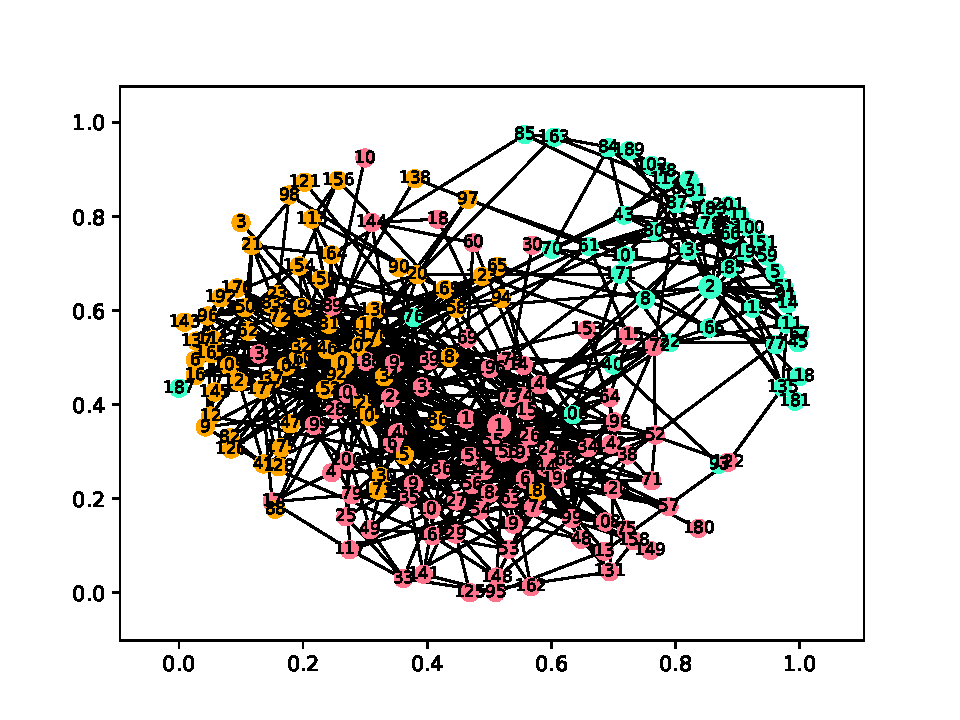
\includegraphics[trim={1cm .5cm 1cm 1cm}, clip, width=\linewidth]{img/pdf/plot-0200.pdf} 
    \caption{200 cycles}
    \label{fig:200}
  \end{subfigure}

  \vspace{0cm}

  \begin{subfigure}[t]{.45\textwidth}
    \centering
    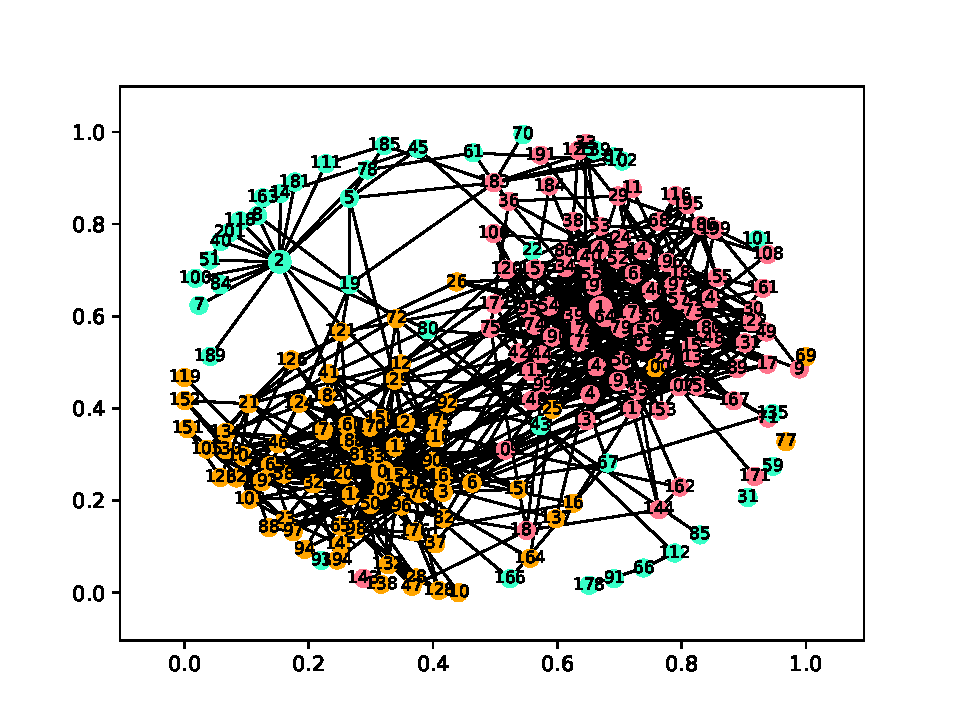
\includegraphics[trim={1cm .5cm 1cm 1cm}, clip, width=\linewidth]{img/pdf/plot-0400.pdf} 
    \caption{400 cycles}
    \label{fig:400}
  \end{subfigure}
  \begin{subfigure}[t]{.45\textwidth}
    \centering
    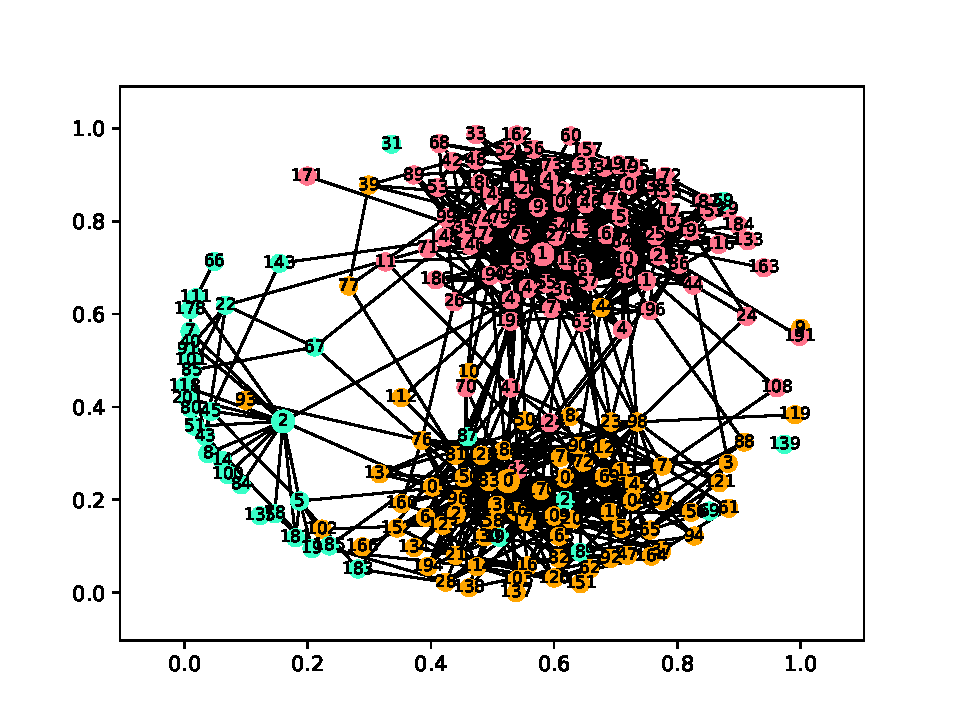
\includegraphics[trim={1cm .5cm 1cm 1cm}, clip, width=\linewidth]{img/pdf/plot-0500.pdf} 
    \caption{500 cycles}
    \label{fig:500}
  \end{subfigure}
 
  \caption{Plot at different final time steps for a simulation with 3 sources, 200 users, initial average degree of users 3 and 500 time steps. Random seed initialized to 17.}
\end{figure}

\subsection{After the simulation: what to notice}\label{subsec:after}
We show graphs of a previous run: the parameters used are, seed 17, 3 sources,
200 users, initial average degree of 3, and 500 time steps.
In figure~\ref{fig:1} we see the net during initialization. Diffusion
has not started yet and users are mostly inactive:
sources have create one news and the few active users are unaware.
After five time steps, figure~\ref{fig:5}, some users have changed their state
to active and started to spread. However, a few of blue users uninformed still remain.
At thenth iteration, in figure~\ref{fig:10}, almost every user
has a news inside and the whole network might a well be homogeneously mixed. 
We have also the first edge creation and remotion, 
consequntly the network's topology start to changing.
Now we jump to the fiftieth iteration, figure~\ref{fig:50},to see that
all the users except one are involved in the dynamic. There is still no
clue of segregation.
After another fifty steps we detect the first clear symptom of segregation.
Moving on of a hundred in a hundred time steps, we see how the orange news
is inclined to disappear and arise a strong segregation in two communities
 due to past influence between users.

\subsection{Further implementations}\label{subsec:implementations}
Some possible future developments are:
\begin{itemize}
\item [adding and removing nodes during execution] can yield big changes
  in the process;
  \item [different algorithm of net generation] at initial clock could be implemented e.g. Barabasi-Albert algorithm or Watts-strogatz algorithm;
\item [look for emerging network behaviors] as said in \textit{\nameref{sec:introduction}} we hope to point out scale-free regime;
\item [analyze the activation time] starting from microscopic behaviors
  it is possible to reproduce macroscopic phenomena such as bursty
  patterns.\cite{goh_burstiness_2008}
\end{itemize}

\subsection{Conclusion}\label{subsec:conclusion}
%
%We would like to emphasize that our model of spreading of news is not based
%on some epidemic model e.g. SIR or another version governed by differential
%equations. The model instead can be to see like an intersection between
%a theshold method and a cascade model, founded on microscopic actions made
%available to agents  and based on the common sense and the social realities,
%for example the RICH PHENOMENON .. mancanza smetto quas
%
%
%La particolarità del modello puo' essere svelata da semplici osservazioni: più notizie possono diffondersi nella rete e coesistere nella
% dinamica di diffusione; le notizie sono generate da sources che sono parte integrante della rete; si modellizza una memoria individuale
% di ogni agente che gli consente di ricordare un certo numero di news diffuse; si modellizza l'influenza sociale che modifica lo stato mentale;
%
% \\
 We expect that memory length will lead to measurable macroscopic
 dynamical effects: this is what we would like to investigate.
 This project will advance our understanding on this hypotesis:
 several simulations, performed with different parameters, could lead
 us to a proof which decides the conjecture.
 We observed segregation in almost all examples and some parameters might be
 more relevant than others. Two open problems arise: which are the key ones
 and, if we found them out, which their values or their ranges would be.
 This is pure speculation on our part but if it were right we could
 state which parameters are crucial.
 A second issue we have previously discussed is the emerging scale
 free dynamic: the authenticity of our guess will be validated
 through statistical observations.
 
